% article.tex, a sample LaTeX file.
% Run LaTeX on this file twice for proper section numbers.
% A '%' causes LaTeX to ignore remaining text on the line

% Use the following line for draft mode (double spaced, single column)
\documentclass[preprint,pre,floats,aps,amsmath,amssymb]{revtex4}

% Use the following line for journal mode (single spaced, double column)
%\documentclass[twocolumn,pre,floats,aps,amsmath,amssymb]{revtex4}
% \usepackage{geometry}
\usepackage{graphicx}
\graphicspath{{G:/Dev/sabr_val/src/doc/charts/}}
\usepackage{physics}
\usepackage{bm}
\usepackage{amsmath} 
\numberwithin{equation}{section} 
\makeatletter
\@addtoreset{equation}{section}
\makeatother

\begin{document}

\title{SABR model IR swaptions calibration, vol cube interpolation and risk.}
\author{Valeriu Biniuc}
\date{\today}

\begin{abstract}
This note  describes SABR model specification and IR swaption volcube calibration, pricing and risk management.
\end{abstract}

\maketitle

\section{The SABR model specification}
\label{sec:intro}
For interest rates original SABR model was extended to handle negative rates using either Normal SABR or Shifted SABR dynamics see \cite{MVS}.

\begin{flalign*}
dF_{t} &= \alpha_{t}(F_{t}+o)^{\beta}dW_{t} \\
d\alpha_{t} &= \nu\alpha_{t}dZ_{t} \\
dW_{t}dZ_{t} &= \rho dt \\
\end{flalign*}

where the following 5 parameters are defined as following : $0\leq\beta\leq1$ , $0<rho<1$ ,  $o \geq 0$ , $\nu \geq 0$ ,$\alpha_{0}>0$. 

Setting $\beta=0$ the model reduces to Normal SABR model.The normal basis point vol is expressed as follows:

\begin{flalign*}
\sigma_{N}(K) &= \alpha_{0}\frac{\zeta}{\chi(\zeta)}\left( 1+\frac{2-3\rho^{2}}{24}\nu^{2}T\right) \\
\zeta_{t} &= \frac{\nu}{\alpha_{0}}\left(F-K\right) \\
\chi(\zeta) &= \log\left(\frac{\sqrt{1-2\rho\zeta+\zeta^{2}}-\rho+\zeta}{1-\rho}\right) \\
\end{flalign*}

and atmf basis point vol is
\begin{flalign*}
\sigma_{N}(F) &= \alpha_{0}\left( 1+\frac{2-3\rho^{2}}{24}\nu^{2}T\right) \\
\end{flalign*}

\section{Calibration methodology}

Calibration methodology consists in 3 steps: \\
- Setting user defined parameters ($o$, $\beta$)\\
- Calibration approach of $\alpha_{0}$, $\rho$ and $\nu$ \\
- Parameter interpolation across non standard expiry and tenors. \\


\subsection{User defined parameters}

Due to over-parametrization of skew parameters ($o$, $\beta$ and $\rho$), rate traders usually specify for each Expiry and Tenor 2 skew parameters shift $o$, $\beta$ and calibrate the other 3 parameters: $\alpha_{0}$, $\rho$ and $\nu$.  Positive shift parameter is used to deal with zero absorbing boundary condition and allow for negative rates when $0<\beta<=0.5$. We set by default shift $o$ and $\beta$ levels to 0  which is SABR normal.


\subsection{Sequential calibration approach}

In order to achieve exact calibration of ATMF normal volatility, we calibrate the 3 remaining parameters sequentially. $\rho$ and $\nu$ are calibrated by best fit minimising the discrepancy between market normal volatilities and model. And $\alpha_{0}$ is implied from ATMF normal volatility solving the cubic polynomial in $\alpha_{0}$ below. For more details see \cite{ExpSABR}.


For $0<\beta\leq 1$, atmf normal basis point vol can be expressed as a cubic polynomial in $\alpha_{0}$.

\begin{flalign*}
\sigma_{N}(F) &= \alpha_{0}(F+o)^{\beta}\left(\left( 1+\frac{2-3\rho^{2}}{24}\nu^{2}T\right)+\frac{\rho\nu\beta T}{4(F+o)^{1-\beta}}\alpha_{0}+\frac{\beta(\beta-2)T}{24(F+o)^{2-2\beta}}\alpha_{0}^{2}\right) \\
\end{flalign*}



Figure \ref{fig:swaptions_calibration_results} shows swaptions bp vol calibration results for Expiry and Tenor.


\begin{figure}[t!]
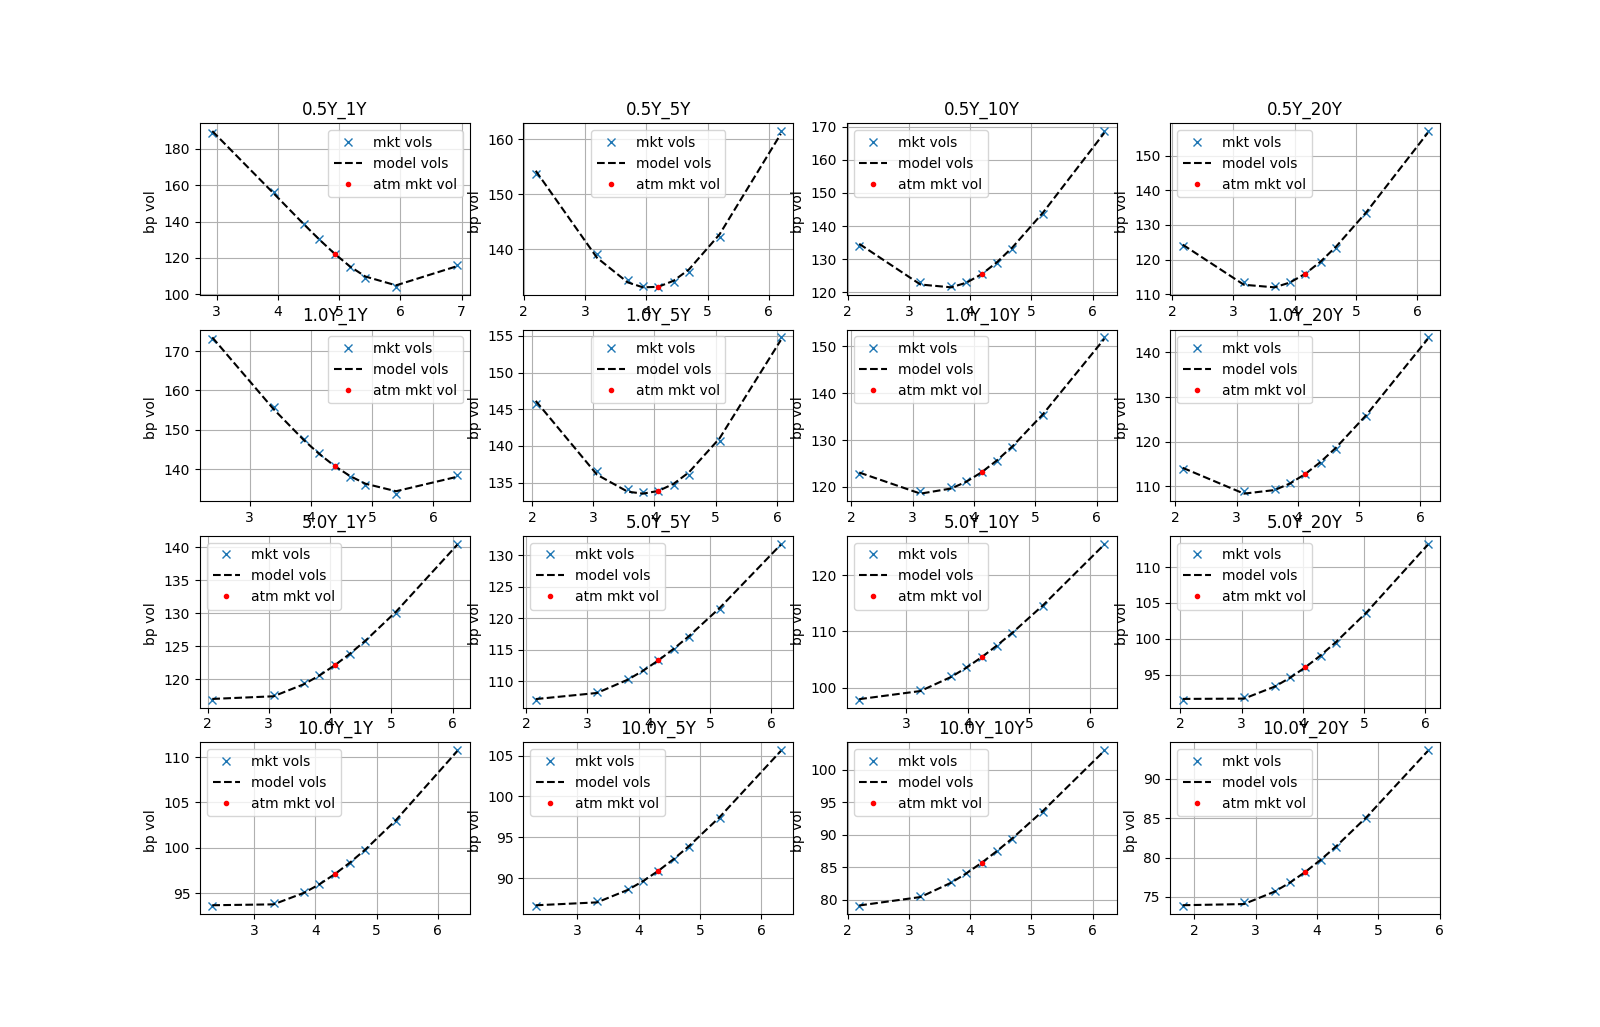
\includegraphics[width=\linewidth]{swaptions_calibration_results.png}
  \caption{Swaptions calibration results in bp vol.}
  \label{fig:swaptions_calibration_results}
\end{figure}

\begin{figure}[t!]
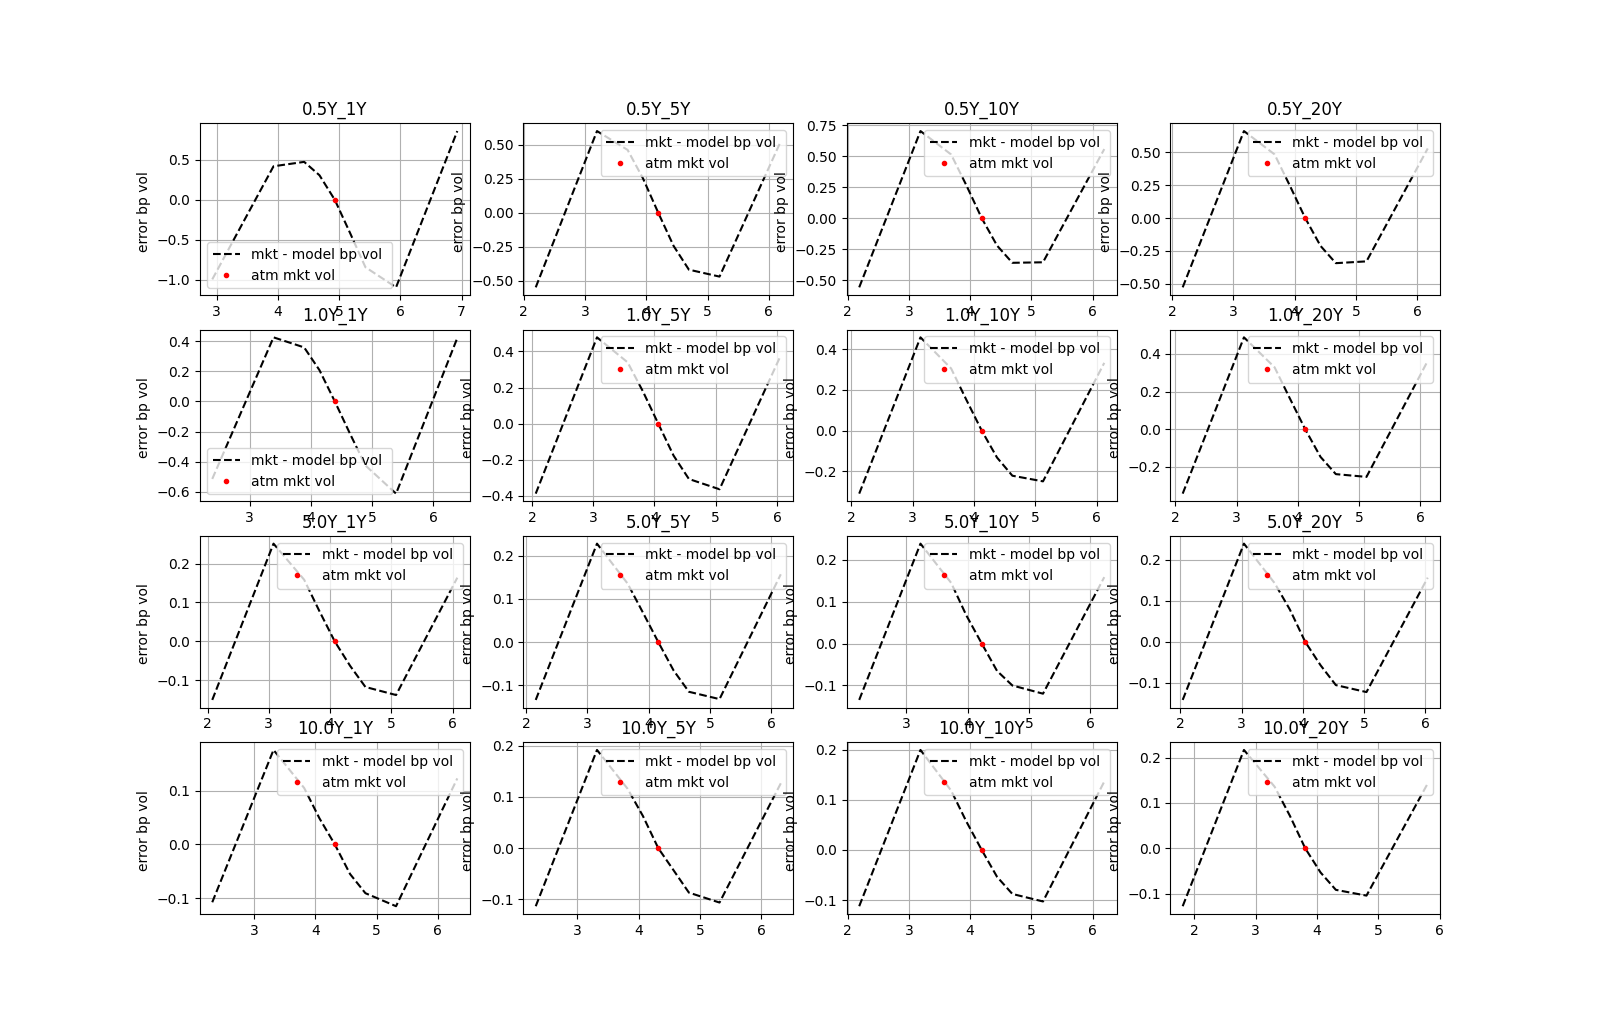
\includegraphics[width=\linewidth]{swaption_calibration_errors_bps.png}
  \caption{Swaptions calibration errors in bp vol.}
  \label{fig:swaptions_calibration_errors}
\end{figure}

As one can see in Figure \ref{fig:swaptions_calibration_errors} below, calibration error of ATMF normal vol are always zero.



\subsection{IR SABR vol cube parameter interpolation approach}

First, we use bilinear interpolation by Expiry and Tenor for shift $o$, $\beta$, $\rho$ and $\nu$ parameters. \\
Second, we interpolate ATMF normal volatility linearly in Tenor and linear ATMF term variance interpolation in expiry as follows: \\

Assume, we found ATMF normal volatility for 2 adjacent expiries $t\in[t_{i},t_{i+1}]$ and corresponding ATMF normal vols $\sigma_{N}(F_{t_{i}})$ and $\sigma_{N}(F_{t_{i+1}})$. The ATMF  normal vol for expiry $t$ is calculated as follows: \\

\begin{flalign*}
\sigma_{N}(F_{t}) &= \sqrt{\left(\sigma_{N}(F_{t_{i}})^{2} t_{i} \times (1-dt) + \sigma_{N}(F_{t_{i+1}})^{2} t_{i+1}  \times dt\right)/t} \\
\end{flalign*}

where,
\begin{flalign*}
dt &= \frac{t-t_{i}}{t_{i+1}-t_{i}} \\
\end{flalign*}


After, we imply from ATMF normal volatility the corresponding $\alpha_{0}$ using same cubic polynomial formula as above.


\section{Swaptions pricing and Hedging in SABR Normal}

Swaption pricing is computed using Bachelier Normal model using SABR normal volatility for a given expiry, strike and underlying. 


\subsection{IR swaption pricing}

\begin{flalign*}
Swpt(F_{t,T},K,\sigma_{N}(F_{t,T},K,t),cp) &= PV01(0,t,T) \times \sigma_{N}(F_{t,T},K,t)\sqrt{t}\left(d \times N(d)+n(d)\right)\\
cp &= +1 \text{ for pay otherwise -1 receive} \\
d &=  cp \times\frac{F-K}{\sigma_{N}(F_{t,T},K,t)\sqrt{t}}\\
PVO1(0,t,T) &= \text{ is the  swap numeraire or PVO1} \\
\end{flalign*}


Example 1) \\
Price a 10m USD receiver swaption expiring in 2Y into 8Y swap  ATM+50bps

\begin{flalign*}
\text{Fwd}(2Y,8Y) = 0.04068\\
\text{Strike} = 0.04568 \\
\text{PVO1}(2Y,8Y)= 6.1628\\
\sigma_{N} = 120.63 \text{ bps} \\
\text{SABR params} \\
\alpha = 0.011131 \\
\rho = 0.267 \\
\nu = 0.5331 \\
\text{PV} = 591,375 \text{ USD}
\end{flalign*}



Example 2) \\
Price a 10m USD payer Swaption 5Yr expiry into 5Y swap ATM -75bps

\begin{flalign*}
\text{Fwd}(5Y,5Y) = 0.04157\\
\text{Strike} = 0.03407\\
\text{PVO1}(5Y,5Y)= 3.6162\\
\sigma_{N} = 109.09 \text{ bps} \\
\text{SABR params} \\
\alpha = 0.010882 \\
\rho = 0.37676 \\
\nu = 0.35499 \\
\text{PV} = 504,022 \text{ USD}
\end{flalign*}


\subsection{IR swaption Delta, Vega risk adjustments}

The are 2 well known delta and vega risk adjustments applied to SABR model (Black or Normal). \\
In the first approach, forward rate and model volatility move independently. \\ 
In the second approach, we take into account the average correlation effect between forward and volatility, It was developed by Bartlett and extended by Hagan later.  For more details see \cite{HedgingSABR} \\

For simplicity we write implied normal vol at the strike $\sigma_{N} :=\sigma_{N}(F_{t,T},K,t)$ and $\sigma_{N}^{atm} :=\sigma_{N}(F_{t,T},F_{t,T},t)$ as atmf implied normal volatility. \\

In the first approach, SABR delta is adjusted by the change in the option implied volatility due to change in the underlying forward rate. And SABR vega is adjusted by the change in normal SABR vol due to change in initial model vol $\alpha_{0}$ As follows:

\begin{flalign*}
\frac{\partial Swpt}{\partial F} &= \Delta_{SABR} = \Delta_{N} +\frac{\partial Swpt}{\partial \sigma_{N}} \frac{\partial \sigma_{N}}{\partial  F} = \Delta_{N} + \text{Vega}_{N} \frac{\partial \sigma_{N}}{\partial  F}\\
\frac{\partial Swpt}{\partial \alpha_{0}} &=\text{Vega}_{SABR} =  \frac{\partial Swpt}{\partial \sigma_{N}} \times \frac{\partial \sigma_{N}}{\partial \alpha_{0}} =\text{Vega}_{N} \times \frac{\partial \sigma_{N}}{\partial \alpha_{0}}  \\
\end{flalign*}


In the 2nd approach, stoch vol dynamics can be rewritten as correlated part of underlying forward rate driver and orthogonal part.


\begin{flalign*}
dF_{t} &= \alpha_{t}(F_{t}+o)^{\beta}dW_{t} \\
d\alpha_{t} &= \nu\alpha_{t}dZ_{t} =  \nu\alpha_{t}\left(\rho dW_{t} +\sqrt{1-\rho^{2}}dZ_{t}\right) = \frac{\rho \nu}{(F_{t}+o)^{\beta}} dF_{t} +\nu \alpha_{t}\sqrt{1-\rho^{2}}dZ_{t}\\
\end{flalign*}

Thus the average change in $\alpha$ due to change in the forward is 


\begin{flalign*}
d\alpha_{t} &= \frac{\rho \nu}{(F_{t}+o)^{\beta}} dF_{t} \\
\end{flalign*}


In the same way, we can rewrite the change in forward underlying dynamics in term of volatility change.


\begin{flalign*}
dF_{t} &= \alpha_{t}(F_{t}+o)^{\beta}dW_{t} = \alpha_{t}(F_{t}+o)^{\beta} \left(\rho dZ_{t} + \sqrt{1-\rho^{2}}dW_{t}\right) = (F_{t}+o)^{\beta} \left(\frac{\rho}{\nu} d\alpha_{t} + \alpha_{t} \sqrt{1-\rho^{2}}dW_{t}\right)\\
d\alpha_{t} &= \nu\alpha_{t}dZ_{t} \\
\end{flalign*}


Thus the average change in the forward rate due to change in the $\alpha$ is 


\begin{flalign*}
dF_{t} &= \frac{(F_{t}+o)^{\beta} \rho}{\nu} d\alpha_{t} \\
\end{flalign*}



The new Bartlett's adjusted delta and vega will take into account the change in normal vol due to change in volatility and forward as follows.



\begin{flalign*}
\Delta_{SABR} &= \Delta_{N} + \text{Vega}_{N} \left(\frac{\partial \sigma_{N}}{\partial  F} + \frac{\partial \sigma_{N}}{\partial  \alpha} \frac{\partial \alpha}{\partial  F} \right)=  \Delta_{N} + \text{Vega}_{N} \left(\frac{\partial \sigma_{N}}{\partial  F} + \frac{\partial \sigma_{N}}{\partial  \alpha} \frac{\rho \nu}{(F_{t}+o)^{\beta}} \right)\\
\text{Vega}_{SABR} &= \text{Vega}_{N} \left( \frac{\partial \sigma_{N}}{\partial \alpha} \right)=\text{Vega}_{N} \left( \frac{\partial \sigma_{N}}{\partial \alpha} + \frac{\partial \sigma_{N}}{\partial  F} \frac{\partial F}{\partial  \alpha} \right) = \text{Vega}_{N} \left( \frac{\partial \sigma_{N}}{\partial \alpha} + \frac{\partial \sigma_{N}}{\partial  F} \frac{(F_{t}+o)^{\beta} \rho}{\nu} \right)   \\
\end{flalign*}


In our SABR Normal calibration approach, $\sigma_{N}^{atm}$ stays constant as other SABR parameters change. As a result, using chain rule approach on $\frac{\partial \sigma_{N}}{\partial F} = \frac{\partial \sigma_{N}}{\partial \sigma_{N}^{atm}} \frac{\partial \sigma_{N}^{atm}}{\partial F} = 0 $ .

Thus the 2 approaches simplify as follows:


In the 1st approach, Normal swaption delta stays unchanged and only vega is adjusted.

\begin{flalign*}
\frac{\partial Swpt}{\partial F} &= \Delta_{SABR} = \Delta_{N} +\frac{\partial Swpt}{\partial \sigma_{N}} \frac{\partial \sigma_{N}}{\partial  F} = \Delta_{N} \\
\frac{\partial Swpt}{\partial \alpha_{0}} &=\text{Vega}_{SABR} =  \frac{\partial Swpt}{\partial \sigma_{N}} \times \frac{\partial \sigma_{N}}{\partial \alpha_{0}} =\text{Vega}_{N} \times \frac{\partial \sigma_{N}}{\partial \alpha_{0}}  \\
\end{flalign*}


In the 2nd approach, which is used in our implementation, Vega adjustment stays the same as in the first approach and only delta adjustment applies to account for the correlated volatility change due to the move in forward rate.


\begin{flalign*}
\Delta_{SABR} &= \Delta_{N} + \text{Vega}_{N} \left(\frac{\partial \sigma_{N}}{\partial  F} + \frac{\partial \sigma_{N}}{\partial  \alpha} \frac{\partial \alpha}{\partial  F} \right)=  \Delta_{N} + \text{Vega}_{N} \frac{\partial \sigma_{N}}{\partial  \alpha} \frac{\rho \nu}{(F_{t}+o)^{\beta}}\\
\text{Vega}_{SABR} &= \text{Vega}_{N} \left( \frac{\partial \sigma_{N}}{\partial \alpha} \right)=\text{Vega}_{N} \left( \frac{\partial \sigma_{N}}{\partial \alpha} + \frac{\partial \sigma_{N}}{\partial  F} \frac{\partial F}{\partial  \alpha} \right) = \text{Vega}_{N} \frac{\partial \sigma_{N}}{\partial \alpha}  \\
\end{flalign*}



Please note that Delta, Vega and Gamma have to be scaled by 10000 to get 1bp change in rate, vol.
 

\subsection{IR swaption Theta}

IR swaption $\Theta$ can be decomposed in 3 parts: \\
- Sensitivity in optice price due to time decay, usual Bachelier theta \\
- Sensitivity in option price due to expiry change (SABR parameters interpolation change next business day) \\
- Carry or PV accrual of the trade \\


1) Price and risk of 10m  USD receiver swaption expiring in 2Y into 8Y swap  ATM+50bps \\

- PV = 591,375 USD \\
- Delta = -33,009,822 USD or -3,301 USD per 1 bp rate change \\
- Vega = 34,474,364 USD or 3,447 USD per 1 bp change in alpha \\
- Gamma = 1,380,596,359 USD or Delta will change 138,060 USD for 1bp rate change \\
- Theta = -49,401 USD or a decay of -135 USD for 1 calendar day.  $dt = 1/365$ \\


2 ) Price and risk of 10m USD payer Swaption 5Yr expiry into 5Y swap ATM -75bps \\

- PV = 504,022 USD \\
- Delta = 26,692,228 USD or 2,669 USD per 1 bp rate change \\
- Vega = 31,734,512 USD or 3,173 USD per 1 bp change in alpha \\
- Gamma = 564,118,187 USD or Delta will change 56,411 USD for 1bp rate change \\
- Theta = -1,937 USD or a decay of -5 USD for 1 calendar day. $dt = 1/365$ \\



\section{Pricer tool for swaptions structures (flys, spreads, calendar spreads, calendar straddles, etc...)}

I would recommend to have a tool where we can see pv, risk for each individual leg and the pv and risk of the aggregated package.

For instance, a long payer spread is long payer at strike K1 and short payer at higher strike K2. We need to be able to see pv and risk on each leg and save the package as a package with a ticker.

At the same time, it should be possible to aggregate multiple options and underlyings in the packaged. For instance, delta neutral payer/receiver spread, will take a payer/reicever spread and an underlying swap.


For simple structures such as swap spreads, flys or exchange traded options spreads, flys we could run some additional statics on the package:
- is the package statistically cointegrated
- is the package statistically mean reverting and how fast (mean reversion time)
- display z-scores in bps or standard deviations


\section{IR SABR project description}

\subsection{python code}

It has 2 modules: \\
- ircurves module contains ircurve.py . it calibrates yield curve, computes discount factors, swap rate and swap pvo1. \\
- models module contains 2 files: bachelier.py which builds bachelier model and computes pv and risk. sabr.py with has 2 classes sabr normal formula, and irSabrVolCube volcube. ir volcube fits swaption calibration instruments, interpolates parameters, computes swaption price and risk

Ircuve curve takes a dataframe object of the yield curve and returns ircurve object instance. Ircurve calibration is done by bootstrapping using one to one mapping between swap instrument and discount factor. \\
Zero coupon bond are log linearly interpolated between 2 calibrated maturites, as follows: \\

\begin{flalign*}
D_{t}=D(t_{i})^{1-dt} \times D(t_{i+1})^{dt} \\
\text{ where,} t\in[t_{i},t_{i+1}] \\
\text{and, } dt = \frac{t-t_{i}}{t_{i+1}-t_{i}} \\
\end{flalign*}


irSabrVolCube takes ir mkt vols instruments as a dataframe (Expiry/Tenor, Moneyness) .instance of calibrated ircurve object, default sabr params and left/right extrapolation booleans.

Examples of ir data and ir vols are stored in data folder of the project.


\subsection{Documents, charts, papers}

IR SABR project reference papers, doc and charts are stored in doc folder of the project.


\subsection{Code build and dist}


The code is self contained. It order to run it, please : \\
1) go to \text{sabr val} folder which contain setup.py and run the compand line python setup.py \text{bdist wheel}.
2) go to dist subfolder of the project and run the command line pip install \text{sabr val-0.0.5-py3-none-any.whl}



\begin{thebibliography}{99}


\bibitem[HaganVolSurfaces2018]{MVS} P. Hagan, A.Lesniewski, D. Woodward {\it Managing vol surfaces} (Wilmott magazine. January, 2018).

\bibitem[ExplicitSABRFloch2014]{ExpSABR} F. Le Floch, Gary Kennedy, Explicit SABR Calibration through Simple Expnasions (2014).

\bibitem[HedgingSABRBartlett]{HedgingSABR} Bruce Bartlett, Gorilla Science. Hedging under SABR model. Wilmott magazine

\bibitem[BartlettRiskHagan2016]{SABRriskHagan} P. Hagan, A. Lesniewski. Barlett's Delta in the SABR model. Arxiv.org

\end{thebibliography}

\end{document}             % End of document.

